\documentclass[a4paper,12pt]{article}

\usepackage{amsmath}  % For equations
\usepackage{amsfonts} % For mathematical symbols
\usepackage{graphicx} % For figures
\usepackage{hyperref} % For links
\usepackage{appendix} % For appendices
\usepackage{amssymb}
\usepackage [round,authoryear] {natbib}

\DeclareMathOperator*{\argmax}{argmax}
\DeclareMathOperator*{\argmin}{argmin}

\usepackage{amsthm}
\usepackage{xcolor}

\usepackage{algorithm}
\usepackage{algpseudocode}


\newtheorem{exinn}{Example}
\newtheorem{theorem}{Theorem}
\newtheorem{definition}{Definition}
\newtheorem{axiom}{Axiom}


\title{Sequential Decision-Making for Inventory Control using Bayesian Decision Theory}
\author{Jonas Petersen \\ Ander Runge Walther }
\date{\today}

\begin{document}
	\maketitle
	
	\begin{abstract}
		Inventory control is a core aspect of supply chain management, balancing customer demand fulfillment against the costs of holding and ordering inventory. This paper addresses inventory management through the lens of Bayesian decision theory, enabling probabilistic decision-making under uncertainty. By establishing a framework for sequential decision-making over an infinite time horizon, an optimal solution tailored to a specific asymmetric cost function is derived, offering insights for practical implementations in inventory management.
	\end{abstract}
	
	\section{Introduction}
	Inventory management is a critical component of supply chain management that involves overseeing the ordering, storage, and use of a company's inventory, including raw materials, components, and finished goods. Effective inventory control ensures that a company has adequate stock to meet demand while minimizing costs associated with holding inventory. In practice, this often requires a balance between minimizing stockouts, which disrupt service levels, and limiting overstocking, which incurs unnecessary holding costs.
	
	The coordination of inventory and transportation decisions has gained significant attention over recent decades, driven by the need for specific practices like vendor-managed inventory (VMI), third-party logistics (3PL), and time-definite delivery (TDD) (see, e.g., \citep{CetinkayaLee2000, Alumur2012, Gurler2014}). These programs aim to optimize the balance between inventory holding costs and transportation costs. Traditional inventory models often assume immediate delivery to meet demand, yet this can be inefficient due to the fixed costs of transportation, prompting companies to adopt shipment consolidation policies that merge smaller demands into larger, less frequent shipments \citep{CetinkayaBookbinder2003, HigginsonBookbinder1994}.
	
	Three commonly implemented shipment consolidation policies—quantity-based, time-based, and hybrid—are particularly useful in improving cost efficiency by regulating shipment size or timing. Each policy type has distinct impacts on performance metrics, such as delay penalties, average inventory, and annual costs, guiding companies toward designing more efficient inventory-transportation systems \citep{Cetinkaya2005, Wei2020, Cetinkaya2006}.
	
	While these approaches provide valuable frameworks, they do not explicitly account for the uncertainties inherent in demand fluctuations or the associated asymmetric costs of overstocking and understocking. In settings where inventory decisions must be made sequentially, uncertainty can be more effectively managed through Bayesian decision theory, which offers a probabilistic approach to decision-making under uncertainty. This framework allows for more refined, sequential adjustments to inventory based on demand forecasting, which dynamically incorporates new data over time.
	
	In this study, Bayesian decision theory is utilized to address a sequential inventory control problem. Specifically, an optimal decision-making framework is derived based on a discounted asymmetric cost function, considering the impact of decisions made infinitely far into the future. Our model involves a decision-maker (henceforth referred to as the Robot) who manages stock levels over time in an interactive environment shaped by a random demand process. Through this setup, a mathematically rigorous and computationally feasible solution for optimal inventory decisions that account for uncertainty and asymmetric costs is derived.
	
	\section{Sequential Decision-Making Framework}
	To formalize the sequential decision-making problem, consider a stock management scenario in which the Robot is set in a game against an entity termed Nature, which represents environmental randomness~\citep{lavalle2006}. In this game the Robot and Nature each have to make a decision, $u\in \Omega_U\subset \mathbb{Z}_{\geq 0}$ and $s\in \Omega_S\subset \mathbb{Z}_{\geq 0}$ respectively, for each time step $t\in [1,T]$ ($T\geq L$) into the future. 
	\begin{definition}[Stock level]
		\label{def:stock}
		Given an initial stock $N_0$, the stock level at time $t$ evolves according to
		\begin{equation}
			\begin{split}
				N_t &\equiv N_0 + \sum_{t'=1}^{t} (u_{t'-L} - s_{t'})\\
				& = N_0+\upsilon_t-\zeta_t
			\end{split},
		\end{equation}
		where $u_{t'-L}$ represents the decision made at an earlier time due to a potential lag $L$ and $\zeta_t\equiv \sum_{t'=1}^ts_{t'}$ and $\upsilon_t\equiv \sum_{t'=1}^tu_{t'-L}$. To support probabilistic decision-making, the Robot uses a probabilistic forecast based on data $D$
		\begin{equation}
			p(s_1, s_2, \dots s_T| D, I),
		\end{equation}
		where $I$ denotes any additional background information~\citep{Sivia2006}.
	\end{definition}

	\begin{definition}[Discounted Cost]
		\label{def:cost}
		The Robot receives a numerical penalty, assigned by a cost function, depending on the decisions $\{u\}, \{s\}$ made over the forecast horizon. The cost $C$ is assumed to be discounted and is defined as
		\begin{equation}
			C = \sum_{t=1}^{T} \gamma_{\text{disc}}^{t-1} 
			\left( h_t 1_{N_t > 0} + c_t (1_{N_t > 0} - 1) \right) N_t,
			\label{eq:cost}
		\end{equation}
		where $\gamma_{\text{disc}} \in [0,1]$ is the discount factor, $h_t$ and $c_t$ represent 
		storage (holding) and understocking costs at time $t$, respectively, and 
		$1_{N_t > 0}$ is the indicator function that equals 1 when $N_t > 0$ (see definition \ref{def:stock}) and $0$ otherwise.
	\end{definition}
	
	\begin{definition}[Optimal Policy]
		\label{def:policy}
		Given the data $D$, the Robot’s objective is to formulate a sequence of decision rules, called a policy, $\pi = \{U_0(D)=u_0, U_1(D)=u_1, \dots\}$, where each $U_j(D) = u_j$ minimizes the expected cost (definition \ref{def:cost})
		\begin{equation}
			\pi^* = \arg \min_{\pi} \mathbb{E}[C| D, I]
		\end{equation}
		over the probability distribution of definition \ref{def:stock}. The optimal decisions rules satisfy the first- and second-order conditions
		\begin{equation}
			\begin{split}
				\frac{d}{dU_m} \mathbb{E}[C | D, I] \Big|_{U_m = U_m^*} &= 0 \quad \forall m,\\
				\frac{d^2}{dU_m^2} \mathbb{E}[C | D, I] \Big|_{U_m = U_m^*} & > 0 \quad \forall m.
			\end{split}
			\label{eq:conditions}
		\end{equation}
	\end{definition}

	\begin{theorem}[Optimal Policy Rule for Inventory Control]
		\label{theorem:opt_policy}
		Given the asymmetric cost function of definition \ref{def:cost} the optimal policy (definition \ref{def:policy}) for the Robot at each time step $t$ is defined by (see appendix \ref{app:deriva} for derivation)
		\begin{equation}
			p(N_t^* > 0 | D, I) = \frac{c_t}{c_t + h_t},
			\label{eq:t1}
		\end{equation}
		where
		\begin{equation}
			N_t^* = N_0 +\upsilon_t^*-\zeta_t,
		\end{equation}
		$\zeta_t-\zeta_{t-1}\geq 0$ and $\upsilon_t-\upsilon_{t-1}\geq 0$ by definition. Since negative decisions are not allowed, $\upsilon_t^* = 0$ is the optimal decision in case of $N_t\leq 0$. In this case, the condition in equation \eqref{eq:t1} is not strictly satisfied, as $p(N_t^* > 0 | D, I)$ becomes irrelevant due to the sufficient inventory at time $t$.
	\end{theorem}
	
	
	\section{Optimal Policy under Conditional Independence}
	Equation \eqref{eq:t1} can be written
	\begin{equation}
		\begin{split}
			p(N_t^* > 0 | D, I) &= \sum_{s_1,\dots s_t}1_{N_{t}\geq 0}p(s_1,\dots s_t|D,I)\sum_{s_{t+1},\dots s_T}p(s_{t+1},\dots s_T|s_1,\dots s_t,D,I)\\
			& = \sum_{\zeta_t=0}^{N_0+\upsilon_t}p(\zeta_t|D,I)\sum_{s_{t+1},\dots s_T}p(s_{t+1},\dots s_T|\zeta_t,D,I)\\
		\end{split}
	\end{equation}
	Assuming conditional independence $p(s_{t+1},\dots s_T|\zeta_t,D,I)=p(s_{t+1},\dots s_T|D,I)$
	\begin{equation}
			p(N_t^* > 0 | D, I)  = \sum_{\zeta_t=0}^{N_0+\upsilon_t}p(\zeta_t|D,I).
			\label{eq:indep}
	\end{equation}
	Combining eqation \eqref{eq:indep} with theorem \ref{theorem:opt_policy} implies that the optimal policy is related to quantiles of $\zeta_t$ viz
	\begin{equation}
		\upsilon_t^* = \max(\text{round}(\mathcal{Q}_{\frac{c_t}{c_t+h_t}}\zeta_t-N_0),0),
		\label{eq:opt}
	\end{equation}
	where $\mathcal{Q}_q(X)$ denotes the $q$-quantile of the random variable $X$ and the rounding ensures the decisions belong to $\Omega_U\subset \mathbb{Z}_{\geq 0}$. 
	
	\subsection{Policy Efficiency Ratio}
	In order to gauge the effect of using the optimal policy (equation \eqref{eq:opt}), the associated expected cost can be compared to the expected cost associated to a baseline policy via the policy efficiency ratio (PER)
	\begin{equation}
		\text{PER}\equiv \frac{\mathbb{E}[C|D,I]|_{\pi=\pi^*}}{\mathbb{E}[C|D,I]|_{\pi=\pi'}},
		\label{eq:per_def}
	\end{equation}
	where $\pi^*$ is the optimal policy (theorem \ref{theorem:opt_policy}) and $\pi'$ is the baseline policy. Note that PER$\in [0,1]$ by definition since the optimal policy by definition yield the lowest possible expected cost. Assuming i) $p(\zeta_t|D,I)$ follows a Poisson distribution (with time varying rate parameter) and ii) conditional independence, the expected cost can be written (see appendix \ref{app:expected_cost})
	\begin{equation}
		\begin{split}
			\mathbb{E}[C|D,I] = \sum_{t=1}^{T} \gamma_{\text{disc}}^{t-1} \bigg(& 
			(h_t+c_t)(N_0 + \upsilon_t)\frac{\Gamma(N_0+\upsilon_t+1,\lambda_t)}{\Gamma(N_0+\upsilon_t+1)}\\&- (h_h+c_t)\lambda_t \frac{\Gamma(N_0+\upsilon_t,\lambda_t)}{\Gamma(N_0+\upsilon_t)}\\
			&- c_t(N_0 + \upsilon_t-\lambda_t)\bigg).
		\end{split}
		\label{eq:expected_cost}
	\end{equation}
	Equation \eqref{eq:expected_cost} can be used to calculate the exact PER for any baseline policy.
	
	\subsubsection{Example: Numerical Policy Efficiency Ratio}
	To provide an example of usage of both theorem \ref{theorem:opt_policy} and the PER, the PER is considered with $N_0=37$, $L=6$, constant unit value $c_t=c$, constant holding cost $h_t=h$, Natures decisions shown in figure \ref{fig:ts} and the baseline policy of definition \ref{def:baseline}.
	
	\begin{figure}[h!]
		\centering
		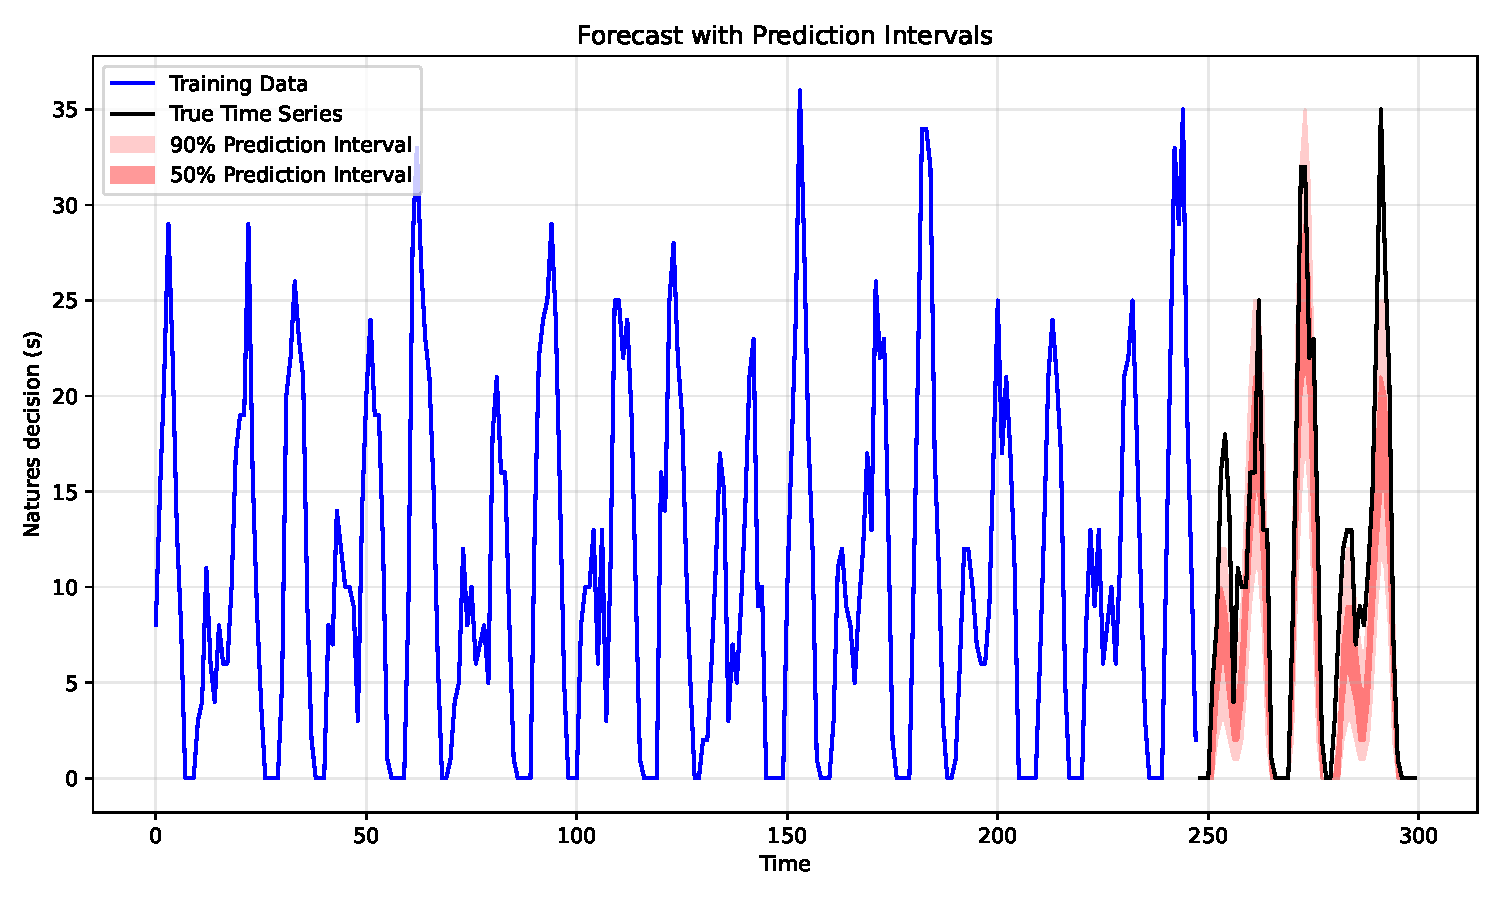
\includegraphics[width=1\textwidth]{figures/time_series.pdf}
		\caption{Natures decisions as a function of time. Blue denotes the historical data available for the Robot, red denote the forecast made by the Robot (based on the historical data) and the black denotes the true future values for reference (not used).}
		\label{fig:ts}
	\end{figure}
	\begin{definition}[Baseline Policy]  
		\label{def:baseline}
		The baseline policy is an $(R, Q)$ inventory policy~\citep{bartmann1992inventory,axsaeter2006inventory}, where the reorder point $R$ determines when to reorder, and the batch quantity, $Q$, is based on the expectation of Natures decisions
		\begin{equation}  
			\upsilon_t' = \max(\text{round}(\mathbb{E}[\zeta_t|D, I] + R - N_0), 0).  
		\end{equation}  
		The rounding ensures the order quantity is an integer, and the maximum function prevents negative orders.
	\end{definition}
		
	Given the above setup, figure \ref{fig:per} presents a heatmap illustrating the Policy Efficiency Ratio (PER) as a function of the reorder point $R$ and the cost-to-holding ratio $\frac{c}{h}$. From the figure, several patterns emerge. In general there seem to be bands of approximately constant PER following $R\sim \ln\frac{c}{h}$ -lines. This band represent the optimal balancing point for $R$ for a given $\frac{c}{h}$. At $\frac{c}{h}=1, R=0$ the PER achieves its maximum at $\simeq 1$, which makes intuitive sense since if $h=c$, the cost function is balanced and the optimal balancing point would be at $R=0$. The maximum value of the band slightly decrease for increasing $\frac{c}{h}$, with PER$\sim 0.9$ as a mean value. Hence, even in case where the reorder point $R$ is optimized perfectly, there is a significantly higher expected cost (around $10\%$) for the baseline (R,Q) - policy relative to the optimal policy (theorem \ref{theorem:opt_policy}). 
	\begin{figure}[h!]
		\centering
		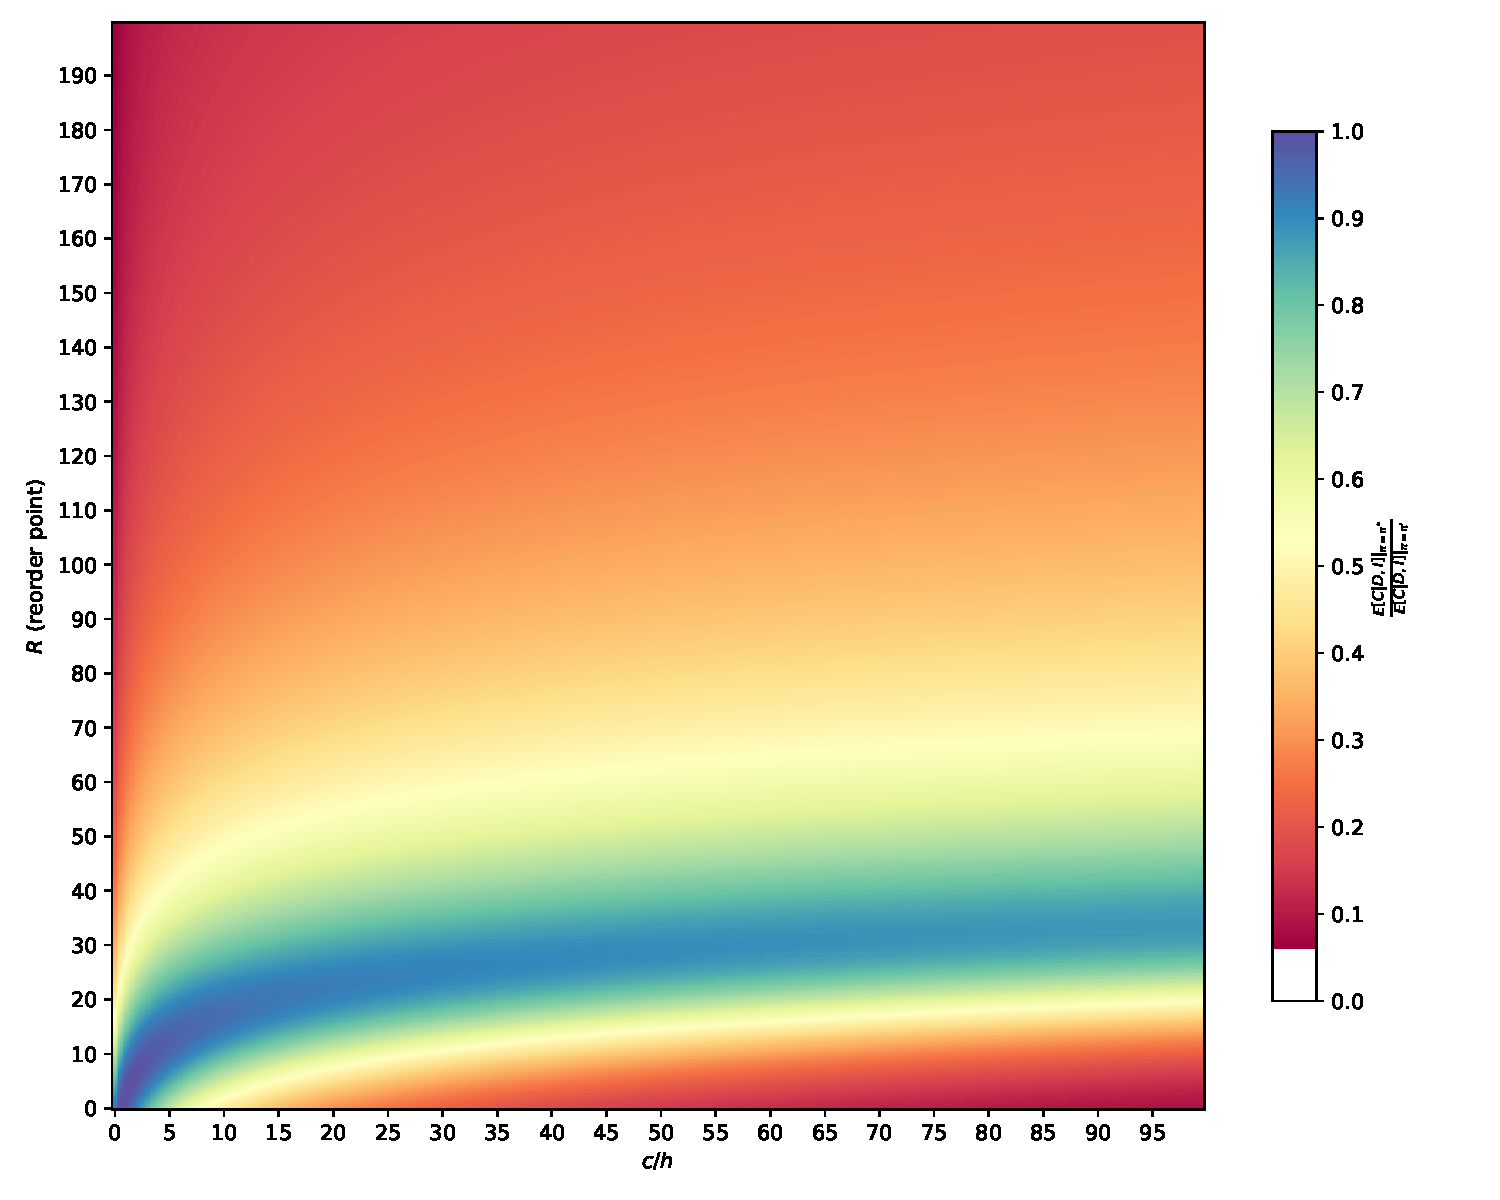
\includegraphics[width=1\textwidth]{figures/per.pdf}
		\caption{Heatmap of the policy efficiency ratio (PER) calculated using equations \eqref{eq:expected_cost}, \eqref{eq:per_def}, definition \ref{def:baseline} and theorem \ref{theorem:opt_policy} with $N_0=37$, $L=6$ and Natures decisions shown in figure \ref{fig:ts}.}
		\label{fig:per}
	\end{figure}

	
	\section{Conclusion}
	Assuming a company has a cost function on the form of definition \ref{def:cost}, they can use the PER in comparison with their current decision policy to i) gauge the expected improvement by implementing the optimal policy or alternatively tune the value of $R$ for their values of $\frac{c}{h}$. The PER shown in figure \ref{fig:per} indicate that for $\frac{c}{h}\gg 1$ the optimal policy yields a reduction of $\sim 10\%$ in expected cost. In case a company is not using decision theory in a formal way, the expected cost reduction may be significantly higher. 
	
	
	
	\newpage
	\begin{appendices}
		\section{Minimization of Expected Cost}
\label{app:deriva}
Define the cost function viz
\begin{equation}
	C = \sum_{t=1}^{\infty}\gamma^{t}(k^\text{sc}_{t}N_{t}^{(+)}+k_{t}^\text{uv}N_{t}^{(-)}),
\end{equation}
where $k^\text{sc}$ and $k^\text{uv}$ represent the "storage cost" and the "unit value". To determine the decision rules, $\xi^*$, that minimize the expected cost $\mathbb{E}[C|D,I]$, the derivative of the cost function with respect to $\xi$ is needed
\begin{equation}
		\frac{dC}{dU_m} = \sum_{t=1}^{\infty}\gamma^{t}\bigg(k^\text{sc}_{t}\frac{dN_{t}^{(+)}}{dU_m}+k_{t}^\text{uv}\frac{dN_{t}^{(-)}}{dU_m}\bigg)
	\label{eq:deriv_1ab}
\end{equation}
where
\begin{equation}
	\begin{split}
		\frac{dN_{t}^{(+)}}{dU_m}& =\sum_q 	\frac{dN_{t}^{(+)}}{dN_q}\frac{dN_q}{dU_m}\\
		& \simeq\sum_q 	1_{N_{t}\geq 0}\delta_{t,q}\frac{dN_q}{dU_m}\\
		& = 1_{N_{t}\geq 0}\sum_{t'=1}^t\frac{dU_{t'-L}}{dU_m}\\
		& = 1_{N_{t}\geq 0}\sum_{t'=1}^t\delta_{t'-L,m},\\
		\frac{dN_{t}^{(-)}}{dU_m} &\simeq (1_{N_t\geq 0}-1)\sum_{t'=1}^t\delta_{t'-L,m},
		\label{eq:deriv_2ab}
	\end{split}
\end{equation}
and it has been used that
\begin{equation}
	\begin{split}
		\frac{dN_t^{(+)}}{dN_t} & =\frac{\beta N_te^{-\beta N_t}}{(1+e^{-\beta N_t})^2}+\frac{1}{1+e^{-\beta N_t}}\\
		& \simeq \frac{1}{1+e^{-\beta N_t}}\\
		&= \sigma(\beta N_t)\\
		&\simeq 1_{N_{t}\geq 0},\\
		\frac{dN_t^{(-)}}{dN_t} & = \frac{\beta N_te^{\beta N_t}}{(1+e^{\beta N_t})^2}-\frac{1}{1+e^{\beta N_t}}\\
		& \simeq -\frac{1}{1+e^{\beta N_t}}\\
		&= \sigma(\beta N_t)-1\\
		& \simeq  1_{N_{t}\geq 0}-1.
	\end{split}
\end{equation}
Using equation \eqref{eq:deriv_2ab} in equation \eqref{eq:deriv_1ab} 
\begin{equation}
	\begin{split}
		\frac{dC}{dU_m} \simeq \sum_{t=1}^{\infty}\gamma^{t}\bigg(k^\text{sc}_{t}1_{N_{t}\geq 0}+k_{t}^\text{uv}(1_{N_{t}\geq 0}-1)\bigg)\sum_{t'=1}^t\delta_{t'-L,m}.
	\end{split}
\end{equation}
For some generic function $g_t$
\begin{equation}
	\begin{split}
		\sum_{t=1}^{\infty}g_t\sum_{t'=1}^t\delta_{t'-L,m} & = g_1\delta_{1-L,m}+g_2(\delta_{1-L,m}+\delta_{2-L,m})+\dots\\
		&=\sum_{t=L+m}^\infty g_t
	\end{split}
\end{equation}
meaning
\begin{equation}
	\frac{dC}{dU_m} \simeq \sum_{t=L+m}^{\infty}\gamma^{t}(k^\text{sc}_{t}1_{N_{t}\geq 0}+k_{t}^\text{uv}(1_{N_{t}\geq 0}-1)).
	\label{eq:deriv_3a}
\end{equation}
Combining equations \eqref{eq:min_exp_cost} and \eqref{eq:deriv_3a}
\begin{equation}
	\sum_{s_1,s_2,\dots}\sum_{t=L+m}^{\infty}\gamma^{t}(k^\text{sc}_{t}1_{N_{t}\geq 0}+k_{t}^\text{uv}(1_{N_{t}\geq 0}-1))p(s_1,s_{2},\dots|D,I)\overset{!}{=} 0\quad \forall m
\end{equation}
The sums can be evaluated viz
\begin{equation}
	\begin{split}
		\sum_{s_1,s_2,\dots}1_{N_{t}\geq 0}p(s_1,s_{2},\dots|D,I) &= p\bigg(\sum_{t'=1}^{t}s_{t'}\leq N_0+\sum_{t'=1}^{t}U_{t'-L}|D,I\bigg)\\
		&= p(N_t\geq 0|D,I),\\
		\sum_{s_1,s_2,\dots}p(s_1,s_{2},\dots|D,I)&=1.\\
	\end{split}
\end{equation}
Let
\begin{equation}
	\psi_t\equiv (k^\text{sc}_{t}+k_{t}^\text{uv})p(N_t\geq 0|D,I)-k_{t}^\text{uv},
\end{equation} 
then
\begin{equation}
	\begin{split}
		\frac{d}{dU_m}\mathbb{E}[C|D,I]& = \sum_{t=L+m}^{\infty}\gamma^{t}\psi_t\\
		&\overset{!}{=} 0\quad \forall m
	\end{split}
\end{equation}
A recursion relation can be derived viz
\begin{equation}
	\begin{split}
		\frac{d}{dU_0}\mathbb{E}[C|D,I] & = \sum_{t=L}^{\infty}\gamma^{t}\psi_t\\
		& =\gamma^{L}\psi_L+\sum_{t=L+1}^{\infty}\gamma^{t}\psi_t\\
		& =\gamma^{L}\psi_L+\frac{d}{dU_1}\mathbb{E}[C|D,I]\\
		& =\gamma^{L}\psi_L+\gamma^{L+1}\psi_{L+1}+\frac{d}{dU_2}\mathbb{E}[C|D,I]\\
		&=\dots\\
		&\overset{!}{=} 0
	\end{split} 
\end{equation}
Since all derivatives are required to be simultaneously zero,
\begin{equation}
	\gamma^{j}\psi_j\overset{!}{=} 0\quad \forall j \Rightarrow \psi_j=0
\end{equation}
meaning
\begin{equation}
	p(N_t^*\geq 0|D,I)=\frac{k_{t}^\text{uv}}{k^\text{sc}_{t}+k_{t}^\text{uv}},
\end{equation}
where
\begin{equation}
	N_t^*\equiv N_0+\sum_{t'=1}^{t}(U_{t'-L}^*-s_{t'})
\end{equation}
denote the units on stock given optimal decisions.

		\section{Cost Efficiency Ratio}
\label{app:cer}
The expected cost
\begin{equation}
	\begin{split}
		\mathbb{E}[C|D,I] &= \sum_{t=1}^{\infty}\sum_{\zeta_t=0}^\infty \gamma_{\text{disc}}^{t} \left( h_t 1_{N_t> 0} + c_t (1_{N_t> 0}-1) \right)N_tp(\zeta_t| D, I)\\
		&= \sum_{t=1}^{\infty}\sum_{\zeta_t=0}^\infty \gamma_{\text{disc}}^{t} \left( (h_t+c_t) 1_{N_t> 0} - c_t  \right)(N_0 + \upsilon_t-\zeta_t)p(\zeta_t| D, I)\\
		&= \sum_{t=1}^{\infty}\sum_{\zeta_t=0}^\infty \gamma_{\text{disc}}^{t} \bigg( 
		(h_t+c_t)(N_0 + \upsilon_t)1_{N_t> 0}\\
		&\qquad\qquad\qquad\quad-(h_t+c_t) 1_{N_t> 0}\zeta_t
		- c_t(N_0 + \upsilon_t)+c_t\zeta_t\bigg)p(\zeta_t| D, I)
	\end{split}
\end{equation}
the relevant terms
\begin{equation}
	\begin{split}
		\sum_{\zeta_t=0}^\infty1_{N_t> 0}p(\zeta_t| D, I) & = \sum_{\zeta_t=0}^{N_0+\upsilon_t} p(\zeta_t| D, I)\\
		&= \frac{\Gamma(N_0+\upsilon_t+1,\lambda_t)}{\Gamma(N_0+\upsilon_t+1)},\\
		\sum_{\zeta_t=0}^\infty1_{N_t> 0}\zeta_tp(\zeta_t| D, I) & = \sum_{\zeta_t=0}^{N_0+\upsilon_t} \zeta_t p(\zeta_t| D, I)\\
		& = \lambda_t \frac{\Gamma(N_0+\upsilon_t,\lambda_t)}{\Gamma(N_0+\upsilon_t)},\\
		\sum_{\zeta_t=0}^\infty\zeta_tp(\zeta_t| D, I) & = \lambda_t,\\
		\sum_{\zeta_t=0}^\infty p(\zeta_t| D, I) & = 1.\\
	\end{split}
\end{equation}
the gamma functions are unpacked by using 
\begin{equation}
	\frac{\Gamma(x,y)}{\Gamma(x)}\approx \frac{1}{1+e^{-m(x-y)}}
\end{equation}
with $m\sim 0.2$ depending on the scale of $y$. This means
\begin{equation}
	\begin{split}
		\sum_{\zeta_t=0}^\infty1_{N_t> 0}p(\zeta_t| D, I) & \approx \frac{1}{1+e^{-m_t(N_0+\upsilon_t+1-\lambda_t)}}\\
		\sum_{\zeta_t=0}^\infty1_{N_t> 0}\zeta_tp(\zeta_t| D, I) & \approx \lambda_t\frac{1}{1+e^{-m_t(N_0+\upsilon_t-\lambda_t)}}\\
	\end{split}
\end{equation}
This means
\begin{equation}
	\begin{split}
		\mathbb{E}[C|D,I] &\approx \sum_{t=1}^{\infty} \gamma_{\text{disc}}^{t} \bigg( 
		(h_t+c_t)(N_0 + \upsilon_t)\frac{1}{1+e^{-m_t(N_0+\upsilon_t+1-\lambda_t)}}\\
		&\qquad\qquad\qquad\quad-(h_t+c_t) \lambda_t\frac{1}{1+e^{-m_t(N_0+\upsilon_t-\lambda_t)}}
		- c_t(N_0 + \upsilon_t-\lambda_t)\bigg)\\
		&\approx \sum_{t=1}^{\infty} \gamma_{\text{disc}}^{t} \bigg( 
		(h_t+c_t)\bigg[\frac{N_0 + \upsilon_t}{1+e^{-m_t(N_0+\upsilon_t+1-\lambda_t)}}- \frac{\lambda_t}{1+e^{-m_t(N_0+\upsilon_t-\lambda_t)}}\bigg]\\
		&\qquad\qquad\qquad
		- c_t(N_0 + \upsilon_t-\lambda_t)\bigg)\\
	\end{split}
\end{equation}

\subsection{Optimal Expected Cost}

\begin{equation}
	\frac{c_t}{c_t+h_t}\approx\frac{1}{1+e^{-m_t(N_0+\upsilon_t+1-\lambda_t)}}\\
\end{equation}

\begin{equation}
	\frac{c_t}{h_t}\approx e^{m_t(N_0+\upsilon_t+1-\lambda_t)}\\
\end{equation}

\begin{equation}
	\upsilon_t\approx \lambda_t-N_0-1+\frac{1}{m_t}\ln\frac{c_t}{h_t} 
\end{equation}

This means

\begin{equation}
	\begin{split}
		\mathbb{E}[C^*|D,I] &\approx \sum_{t=1}^{\infty} \gamma_{\text{disc}}^{t} \bigg( 
		\bigg[(N_0 + \upsilon_t)c_t- \lambda_tc_t\frac{c_t+h_t}{c_t+e^{m_t}h_t}
		\bigg]- c_t(N_0 + \upsilon_t-\lambda_t)\bigg)\\
		&= \sum_{t=1}^{\infty} \gamma_{\text{disc}}^{t} \lambda_tc_th_t\frac{e^{m_t}-1}{e^{m_t}h_t+c_t}\\
	\end{split}
\end{equation}

\subsection{Baseline Expected Cost}

\begin{equation}
	\upsilon_t= \lambda_t+\epsilon_t-N_0
\end{equation}
where $\epsilon_t\leq \lambda_t$

This means

\begin{equation}
	\begin{split}
		\mathbb{E}[C'|D,I] &\approx \sum_{t=1}^{\infty} \gamma_{\text{disc}}^{t} \bigg( 
		(h_t+c_t)\bigg[\frac{N_0 + \upsilon_t}{1+e^{-m_t(\epsilon_t+1)}}- \frac{\lambda_t}{1+e^{-m_t\epsilon_t}}\bigg]\\
		&\qquad\qquad\qquad
		- c_t(N_0 + \upsilon_t-\lambda_t)\bigg)\\
	\end{split}
\end{equation}

\begin{equation}
	\begin{split}
		\mathbb{E}[C'|D,I] \approx \sum_{t=1}^{\infty} \gamma_{\text{disc}}^{t} h_t\epsilon_t
	\end{split}
\end{equation}


\subsection{Cost Ratio}

\begin{equation}
	\frac{\mathbb{E}[C^*|D,I] }{\mathbb{E}[C'|D,I]}\approx \frac{\sum_{t=1}^{\infty} \gamma_{\text{disc}}^{t} \lambda_tc_th_t\frac{e^{m_t}-1}{e^{m_t}h_t+c_t}}{\sum_{t=1}^{\infty} \gamma_{\text{disc}}^{t} h_t\epsilon_t}
\end{equation}
$h_t,c_t\simeq \text{const}$
\begin{equation}
		\frac{\mathbb{E}[C^*|D,I] }{\mathbb{E}[C'|D,I]}\approx \frac{e^{m_t}-1}{e^{m_t}\frac{h}{c}+1}\frac{\sum_{t=1}^{\infty} \gamma_{\text{disc}}^{t} \lambda_t}{\sum_{t=1}^{\infty} \gamma_{\text{disc}}^{t} \epsilon_t}
\end{equation}
Since $\mathbb{E}[C^*|D,I]$ is the minimum expected cost at all times, the ratio must be smaller or equal to $1$, meaning

\begin{equation}
	(e^{m}-1)\frac{\sum_{t=1}^{\infty} \gamma_{\text{disc}}^{t} \lambda_t}{\sum_{t=1}^{\infty} \gamma_{\text{disc}}^{t} \epsilon_t}=1
\end{equation}
Assuming $\lambda_t\sim \epsilon_t$ for simplicity, then $m_t\sim \ln(2)$. This means
\begin{equation}
	\frac{\mathbb{E}[C^*|D,I] }{\mathbb{E}[C'|D,I]}\sim \frac{1}{1+\frac{2h}{c}}
\end{equation}


		\section{Identities Related to the Poisson Distribution}
\label{sec:poisson_identities}
The Poisson distribution with rate parameter $\lambda$ describes the probability of a discrete random variable $\zeta$ taking integer values. Here, some key identities relevant for the PER (equation \eqref{eq:per_def}) are explored. The cumulative probability of observing $\zeta \leq k$ given a Poisson rate $\lambda$ is
\begin{equation}
	\begin{split}
		p(\zeta \leq k | \lambda) &= e^{-\lambda} \sum_{j=0}^k \frac{\lambda^j}{j!}\\
		& = \frac{\Gamma(k+1,\lambda)}{\Gamma(k+1)},
	\end{split}
\end{equation}
where $\Gamma(k+1,\lambda)$ is the incomplete gamma function and $\Gamma(s)$ denotes the complete gamma function
\begin{equation}
	\Gamma(k+1) = k!.
\end{equation}
Similarly, an expression for the conditional expectation of $\zeta$, given that $\zeta \leq k$, can be derived viz
\begin{equation}
	\begin{split}
		\mathbb{E}[\zeta | \zeta \leq k, \lambda] &= e^{-\lambda} \sum_{j=0}^k j \frac{\lambda^j}{j!} \\
		&= e^{-\lambda} \sum_{j=0}^{k} \frac{\lambda^{j}}{(j-1)!} \\
		&= \lambda e^{-\lambda} \sum_{j=0}^{k-1} \frac{\lambda^{j}}{j!} \\
		&= \lambda \frac{\Gamma(k, \lambda)}{\Gamma(k)}.
	\end{split}
\end{equation}
		\section{Notes}
\begin{enumerate}
	\item In order to eliminate $\upsilon_t$ from the optimal policy, the the equation
	\begin{equation}
		\begin{split}
			\sum_{\zeta_t=0}^\infty1_{N_t> 0}p(\zeta_t| D, I)&= \sum_{\zeta_t=0}^{N_0+\upsilon_t} p(\zeta_t|\upsilon_t\geq 0, D, I)\\
			&=\frac{c_t}{c_t+h_t}1_{\upsilon_t\geq 0}
		\end{split}
	\end{equation}
	must be solvable for $\upsilon_t$. 
	
	\item There are differences in the implementation of the policy using the approximation of the Poisson distribution. This implementation is extremely sensitive, because when you roll over time, you slice the distribution in many places and at some point, your slice will end up between a round down and a round up. From that point, the decisions coming after are affected. In terms of the cost function, it can therefore have a relatively significant effect and an approximation that seems excellent on the face, can have unintended effects. This just means the implementation of the policy should always follow the quantile rather than the approximation.
\end{enumerate}

\begin{enumerate}
	\item A few words on the intuitive interpretation of the cost function? The number of units overstocked multiplied with the cost of overstocking per unit. The number of units understocked multiplied with the value of each unit. The latter represents the lost value.
	\item Mention the benefit of the analytical solution; the computation speed relative to a numerical optimization is highly beneficial at scale.
	\item Compress the recursive relation to $m$-notation. 
	\item The baseline policy is an (R,Q) policy with $R =0$ and $Q = \mathbb{E}[s_t|D,I]$.
	\item Is our result in any of the inventory control books?
	\item will the relationship between baseline and optimal policy depend on forecasting method? I would say yes. How do we handle this?
	
	\item if there is around the same cost for over/under stocking, there is a $30-40\%$ reduction in costs with the optimal policy compared to the baseline. In the limit of $c\gg h$, the reduction in cost approach $0\%$ and the gains are minor. This is the relevant limit in most cases, where the value of the unit significantly outweigh the holding cost. This is relevant, however, it is underlined, that the baseline policy is always equal or worse (statistically, meaning the expected cost is always lower. Expected cost is over a distribution. draws from that distribution can fall either way) than the optimal policy. 
	
	\item PER is highly dependent on the policy. If the reference level is moved away from $N_t =0$, for example, the plot completely changes and the blue area shifts to the top left corner.
\end{enumerate}

\begin{enumerate}
	\item \href{https://www.academia.edu/27965536/Inventorycontroltextbook_140429044831_phpapp02_1_}{S. Axsäter. Inventory control}
	\item \href{https://proceedings.mlr.press/v151/kan22a/kan22a.pdf}{Gasthaus paper}
	\item \href{https://arxiv.org/pdf/2012.02392}{inspiration for introduction}
	\item \href{https://arxiv.org/pdf/2310.17168}{probabilistic trucks}
	\item \href{https://arxiv.org/pdf/2310.16096}{Amazon paper} (inspiration)
\end{enumerate}
	\end{appendices}
	
	
	
	\bibliographystyle{plainnat}
	\bibliography{ref}
	
\end{document}